% !TEX root = 00_dmlr_compel.tex
%%%%%%%%%%%%%%%%%%%%%%%%%%%%%%%%%%%%%%%%%%%%%%%%%%%%%%%%%%%%%%%%%%%%%%%%%%%%%%%%
%  Compel: Curating High Quality Pretraining Data for Language Models
%  via Compression Ratios
%  DMLR (Journal of Data-centric Machine Learning Research) submission
%
%  Rebuilt from the double-blind review PDF (compel.pdf, 2025-12-01) because no
%  local .tex source exists on this machine; de-anonymized per DMLR single-blind
%  policy. Author list from Brando's CV (cv_long.tex, "Preprint 2026" entry).
%  Style:   dmlr2e.sty  (official, from https://github.com/JmlrOrg/dmlr-style-file)
%  Bib:     compel_refs.bib (rebuilt from the PDF reference list; placeholder
%           entries "arXiv:2401.xxxxx"-style repaired with real metadata)
%  New for DMLR: Section 4 (theoretical grounding: Shannon / Kolmogorov / MDL),
%  contributions list, Broader Impact, fixed Fig. 3 caption/panel mismatch,
%  deduplicated examples figure (was Figs. 2 and 5), dropped the leftover ICLR
%  template placeholder appendix.
%%%%%%%%%%%%%%%%%%%%%%%%%%%%%%%%%%%%%%%%%%%%%%%%%%%%%%%%%%%%%%%%%%%%%%%%%%%%%%%%

\documentclass[twoside,11pt]{article}
\usepackage{dmlr2e}

\usepackage{amsmath,amsfonts,amssymb}
\usepackage{graphicx}
\usepackage{url}
\usepackage{booktabs}
\usepackage{xcolor}
\usepackage{enumitem}
\usepackage{CJKutf8} % the high-CR example document in Fig.~\ref{fig:examples} is bilingual (Chinese/English)

\graphicspath{{./}{./figures/}}

% Green = improvement over the unfiltered baseline, red = regression (matches the review PDF's tables).
\newcommand{\imp}[1]{\textcolor[HTML]{1A7F37}{\textbf{#1}}}
\newcommand{\reg}[1]{\textcolor[HTML]{B91C1C}{\textbf{#1}}}

% Required by dmlr2e.sty — fill in after the OpenReview submission is created
\def\openreview{\url{https://openreview.net/forum?id=XXXX}}

% Journal heading metadata — fill in at camera-ready
% \dmlrheading{Volume}{Year}{pages}{submitted}{published}{id}{authors}

\ShortHeadings{Curating Pretraining Data via Compression Ratios}{Obbad, Miranda, Hall, Schaeffer, Koyejo \& Liang}

\firstpageno{1}

%%%%%%%%%%%%%%%%%%%%%%%%%%%%%%%%%%%%%%%%%%%%%%%%%%%%%%%%%%%%%%%%%%%%%%%%%%%%%%%%
\begin{document}

\title{Curating High Quality Pretraining Data for Language Models via Compression Ratios}

% TODO(internal-review): confirm author order, middle-initial style, and email handles with Elyas before submitting.
\author{%
  \name Elyas Obbad$^{1}$ \AND
  \name Brando Miranda$^{1}$ \AND
  \name David L.\ W.\ Hall$^{1}$ \AND
  \name Rylan Schaeffer$^{1}$ \AND
  \name Sanmi Koyejo$^{1}$ \AND
  \name Percy Liang$^{1}$ \\
  \addr $^{1}$Department of Computer Science, Stanford University, Stanford, CA 94305, USA \\
  \texttt{\{eobbad, brando9, dlwh, rschaef, sanmi, pliang\}@cs.stanford.edu}
}

\editor{Handling Editor: TBD}

\maketitle

%=========================  Abstract  ==============================%
\begin{abstract}
% CS197 move 1 — problem motivation: data quality gates capability, curation at web scale is compute-prohibitive.
The quality of pretraining data determines the capabilities of language models, yet identifying high-quality data among billions of web documents remains computationally prohibitive.
% CS197 move 2+3 — prior assumption (quality signals need models/heuristics) and the flip: a model-free scalar suffices.
We introduce \textsc{Compel}, a simple and scalable data processing step that isolates high-quality text using lightweight, compression-based signals.
Our key insight is that the compression ratio of text serves as a robust, model-free proxy for information density: low compression ratios typically reflect repetitive or boilerplate content, whereas high ratios may indicate noisy or unnatural text (e.g., HTML spam or phone numbers).
% CS197 move 4 — instantiation: retain documents inside a calibrated compression-ratio band.
\textsc{Compel} improves dataset quality by retaining only those documents whose compression ratios fall within a chosen range, determined empirically from high-quality reference datasets, without relying on additional model training or heuristic classifiers.
% CS197 move 5 — evaluation with concrete numbers.
\textsc{Compel} improves benchmark performance by 0.4--1.1 points across leading open web-scale datasets---DCLM, FineWeb, and FineWeb-EDU---while requiring only a fraction of the computational resources of traditional filtering methods.
% CS197 move 6 — implication: a practical, compute-efficient complement to existing quality controls.
These results show that compression-based filtering is a practical, compute-efficient complement to prevailing quality controls, capable of boosting pretraining data quality at trillion-token scale.
\end{abstract}

\begin{keywords}
pretraining data curation, data quality, data filtering, compression ratio, LZ4, information density, minimum description length, large language models, data-centric machine learning
\end{keywords}

% !TEX root = 00_dmlr_compel.tex
\section{Introduction}\label{sec:intro}

Recent advances in language models have been driven by pretraining on massive web-scale corpora \citep{brown2020language, du2022glam, hoffmann2022training, raffel2020exploring, xie2023dsir}.
However, the sheer size of these datasets---often comprising trillions of tokens---makes efficient data selection both crucial and challenging \citep{albalak2024survey}.

Carefully curated pretraining data improves downstream performance, as shown by corpora like FineWeb-EDU \citep{penedo2024fineweb} and DCLM \citep{li2024datacomp}.
These datasets rely on multi-stage filtering pipelines that combine language identification, duplication and toxicity checks, and scoring heuristics based on LLMs or perplexity \citep{gehman2020realtoxicity, lee2022deduplicating, marion2023less, albalak2024survey}.
While these pipelines are effective, the notion of ``high quality'' remains under-defined, and existing filters often reflect implicit or task-specific assumptions \citep{longpre2023flan}.
As pretraining datasets grow to tens of trillions of tokens, we need fast and interpretable signals to help identify high-quality data at scale.

This raises a core question: \emph{How can we identify high quality data cheaply and quickly?}

\begin{figure}[t]
\centering
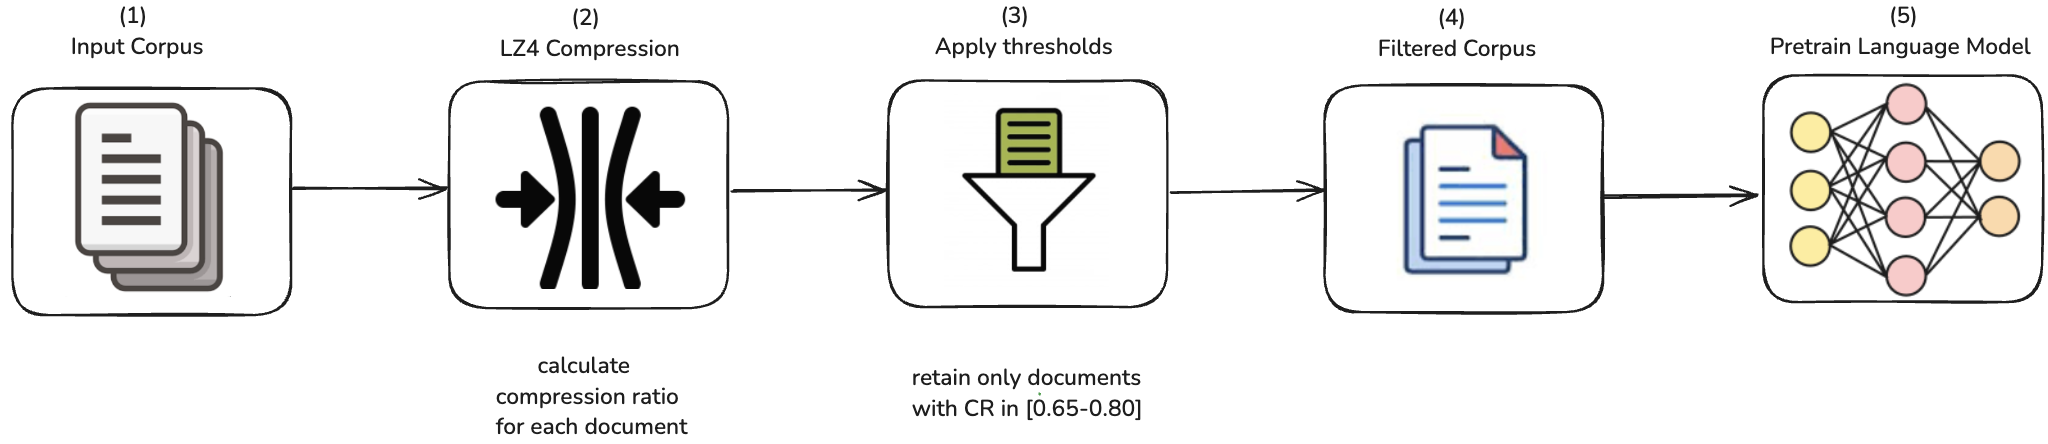
\includegraphics[width=\textwidth]{fig1_pipeline.png}
\caption{\textbf{\textsc{Compel} filters low-quality documents using compression ratio.}
(1) Start with a web-scale input corpus.
(2) Compute the compression ratio (CR) of each document using LZ4 compression.
(3) Discard documents with CR outside a calibrated quality band (e.g., $[0.65, 0.80]$).
(4) Retain the filtered corpus for pretraining.
(5) Pretrain language models with the improved dataset.
\textsc{Compel} improves data quality using a fast, model-free signal that requires no training, inference, or supervision.}
\label{fig:pipeline}
\end{figure}

There are likely many promising answers to this question.
In this work, we introduce an approach that is complementary to existing methods and integrates easily into current filtering pipelines.
We propose \textsc{Compel}, a scalable and lightweight filtering method that uses a document's compression ratio as a proxy for information density (Figure~\ref{fig:pipeline}).
In information theory, data compression encodes information using fewer bits than the original representation, reducing redundancy without losing essential content \citep{shannon1948mathematical}.
Our key insight is that data compression provides a surprisingly effective signal for identifying high-quality text.
Intuitively, well-edited, information-rich documents contain meaningful content that is neither overly repetitive nor excessively noisy.
These documents tend to compress moderately.
In contrast, boilerplate or repetitive content compresses too well (e.g., thousands of identical HTML tags), while noisy or unnatural data compresses poorly due to its lack of structure.
By discarding documents with extremely low or high compression ratios, \textsc{Compel} improves the overall information density of a corpus.
We calibrate filtering thresholds using high-quality reference datasets and show that this lightweight filter can further enhance performance---even when applied on top of state-of-the-art heuristic or model-based filtering.

We validate our method on three leading pretraining corpora---FineWeb, FineWeb-EDU, and DCLM---each of which employs a distinct filtering strategy.
Across 13 downstream tasks, models trained on \textsc{Compel}-filtered data consistently outperform those trained on the original corpora.
These improvements are robust and achieved at negligible computational cost.
The resulting accuracy gains are modest (+0.4--1.1 points), but small, consistent gains from lightweight filters are substantial at scale, offering considerable efficiency benefits on trillion-token datasets \citep{raffel2020exploring, wenzek2020ccnet, ankner2024perplexed}.

\paragraph{Contributions.}
This work contributes to the data side of language-model development:
\begin{itemize}[leftmargin=1.35em,topsep=2pt,itemsep=1pt]
\item A distributional analysis of LZ4 compression ratios across four corpora of varying curation quality (C4, FineWeb-EDU, DCLM, Twitter), showing that higher-quality corpora concentrate in a narrow mid-range band and that this band mirrors the accept/reject decisions of the FineWeb-EDU quality classifier (Section~\ref{sec:cr-signal}).
\item An information-theoretic account of why an interior compression-ratio band should select learnable text, connecting \textsc{Compel} to Shannon entropy, Kolmogorov complexity, and the minimum description length principle (Section~\ref{sec:theory}).
\item \textsc{Compel}, a model-free filter that retains documents whose compression ratio falls in a calibrated band ($[0.65, 0.80]$) and processes over 40{,}000 documents per second on 500 CPUs (Sections~\ref{sec:method}).
\item Pretraining validation at 1.4B and 8B parameters on FineWeb, FineWeb-EDU, and DCLM: macro-average accuracy over 13 benchmarks improves by +1.1, +0.7, and +0.4 points respectively at 1.4B scale, and macro and micro averages also improve at 8B scale (Section~\ref{sec:results}).
\end{itemize}

% !TEX root = 00_dmlr_compel.tex
\section{Related Work}\label{sec:related}

Data selection pipelines for pretraining large models typically involve a sequence of filtering stages to manage the scale and heterogeneity of web-derived corpora.
Common goals include removing undesirable content---such as duplicated boilerplate, SEO spam, or template-heavy pages---and maximizing overall data quality.

\paragraph{Language filtering.}
Language identification is usually performed using lightweight classifiers such as fastText or langdetect \citep{raffel2020exploring, soldaini2024dolma, conneau2019cross, xue2021mt5, laurencon2022roots, grave2018learning}.
These methods are efficient but require careful threshold tuning to avoid excessive false positives or negatives.

\paragraph{Heuristic filtering.}
Surface-level heuristics such as document length or the presence of blacklisted terms are commonly used \citep{rae2021scaling, raffel2020exploring, aghajanyan2022htlm}.
These are computationally cheap but often fail to capture more nuanced indicators of quality.

\paragraph{Quality filtering.}
Retaining educational, human-written text is a key objective in many pipelines.
Classifier-based approaches typically train fastText models or hashed-feature classifiers on curated datasets \citep{du2022glam, longpre2023flan}, while perplexity-based methods score documents using language models trained on high-quality corpora \citep{wenzek2020ccnet, wettig2024qurating}.
Despite strong performance, these methods face limitations: (1) reference corpora may encode cultural or demographic preferences, introducing bias that can marginalize certain dialects, domains, or communities \citep{gururangan2022whose, xu2021detoxifying}, thereby reinforcing existing inequities in model behavior, and (2) the notion of ``quality'' remains inherently subjective and task-dependent \citep{longpre2023flan}.
In contrast, \textsc{Compel} sidesteps these challenges by avoiding reliance on human-annotated or culturally-specific reference corpora, instead using a purely statistical signal (compression ratio) that generalizes across domains.

\paragraph{LM-based quality filtering.}
Recent approaches have employed language models for data refinement.
For instance, \citet{maini2024rephrasing} introduced Web Rephrase Augmented Pre-training (WRAP), which uses instruction-tuned models to paraphrase web documents into styles like Wikipedia or question-answer formats, enhancing data quality and training efficiency.
Similarly, \citet{su2024nemotron} presented Nemotron-CC, a refined dataset derived from Common Crawl, combining classifier ensembling, synthetic data rephrasing, and reduced reliance on heuristic filters to balance data quality and quantity.
While effective, these methods are computationally intensive, requiring substantial resources for model inference and data generation.

\paragraph{Compression-based data selection.}
The link between data compression and language modeling has long been observed \citep{shannon1951prediction}.
Recent studies reinforce this connection: LMs can act as powerful compressors \citep{deletang2023language}, and generalization ability may correlate with compression capacity \citep{huang2024compression}.
\citet{pandey2024gzip} proposes a data-dependent scaling law based on gzip compressibility.
Compression has recently emerged as a scalable, embedding-free signal for data selection and quality estimation.
\citet{yin2024entropy} selects diverse alignment data by scoring examples based on their incremental compressed size, optimizing corpus diversity.
ZIP-FIT \citep{obbad2024zipfit} uses Normalized Compression Distance (NCD) to filter source data for fine-tuning tasks, outperforming neural embeddings in settings such as code and autoformalization.

\textsc{Compel} differs from ZIP and ZIP-FIT in both goal and design.
ZIP aims to construct diverse, low-redundancy subsets for alignment by selecting examples with low incremental compressed size, relying on early-stage training signals and task-specific assumptions.
ZIP-FIT, in contrast, optimizes similarity to a target task distribution using pairwise Normalized Compression Distance.
\textsc{Compel}, by comparison, is a general-purpose filter designed for broad pretraining use: it discards overly redundant or noisy documents based purely on raw compression ratio.
It requires no task-specific supervision, no pairwise comparisons, and no access to model loss signals.
Its simplicity and speed make it especially attractive for trillion-token pipelines.

% !TEX root = 00_dmlr_compel.tex
\section{Compression Ratio as a Signal of Data Quality}\label{sec:cr-signal}

We propose compression ratio as a lightweight, model-free proxy for textual data quality.
Let $x$ be a document and $c(x)$ its compressed representation using a lossless compression algorithm $c$.
We define the \emph{compression ratio} of a string $x$ as:
\begin{equation}\label{eq:cr}
\mathrm{CR}(x) = \frac{\mathrm{num\_bytes}(c(x))}{\mathrm{num\_bytes}(x)},
\end{equation}
where $\mathrm{num\_bytes}(\cdot)$ denotes the number of bytes.
In this work, we use the LZ4 compressor\footnote{\url{https://lz4.github.io/lz4/}}, selected for its speed and streaming compatibility.
While using different compressors is cheap and fast, pretraining LMs is not.
Due to a limited compute budget, we therefore chose to prioritize a single compressor on multiple datasets and multiple language models, over multiple compressors on fewer datasets and LMs, because strong evidence for one compressor is better than weak evidence for multiple compressors.
To the best of our knowledge, our results do not rely on any specifics of LZ4, and so we conjecture that other compressors would work equally well; experiments would be necessary to test this, and we lacked the compute required.

\begin{figure}[t]
\centering
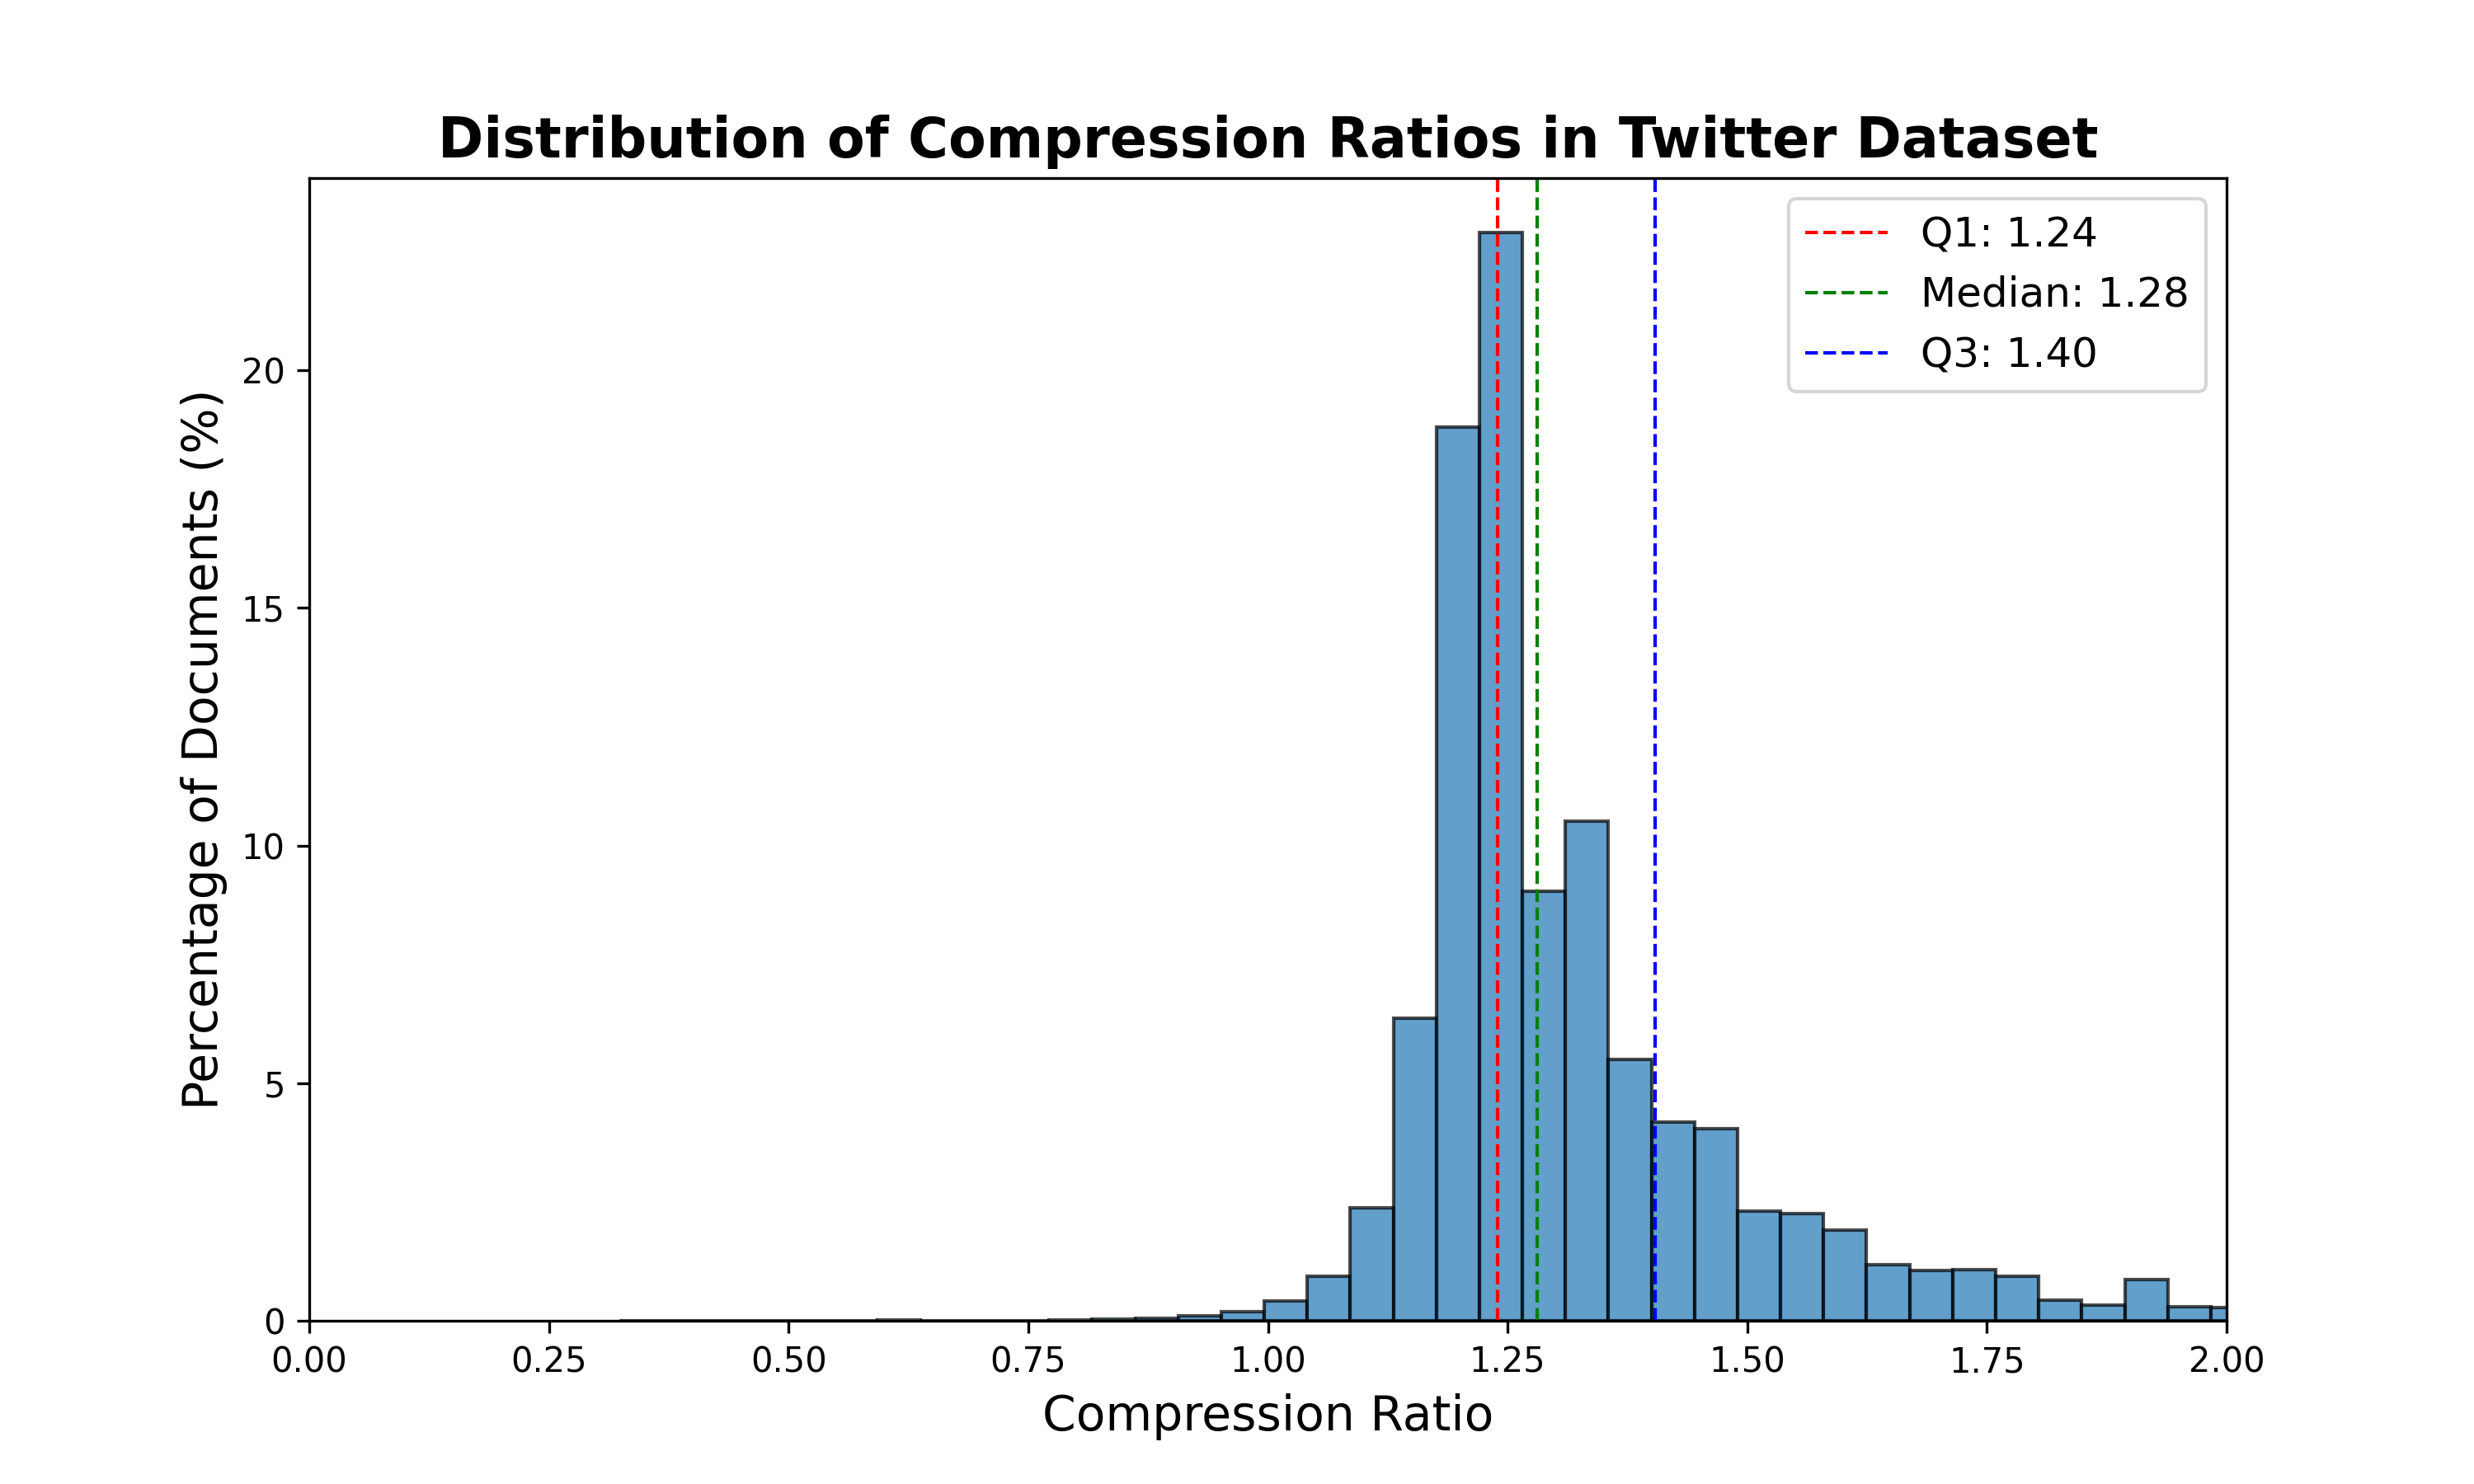
\includegraphics[width=0.49\textwidth]{fig3_cr_twitter.png}\hfill
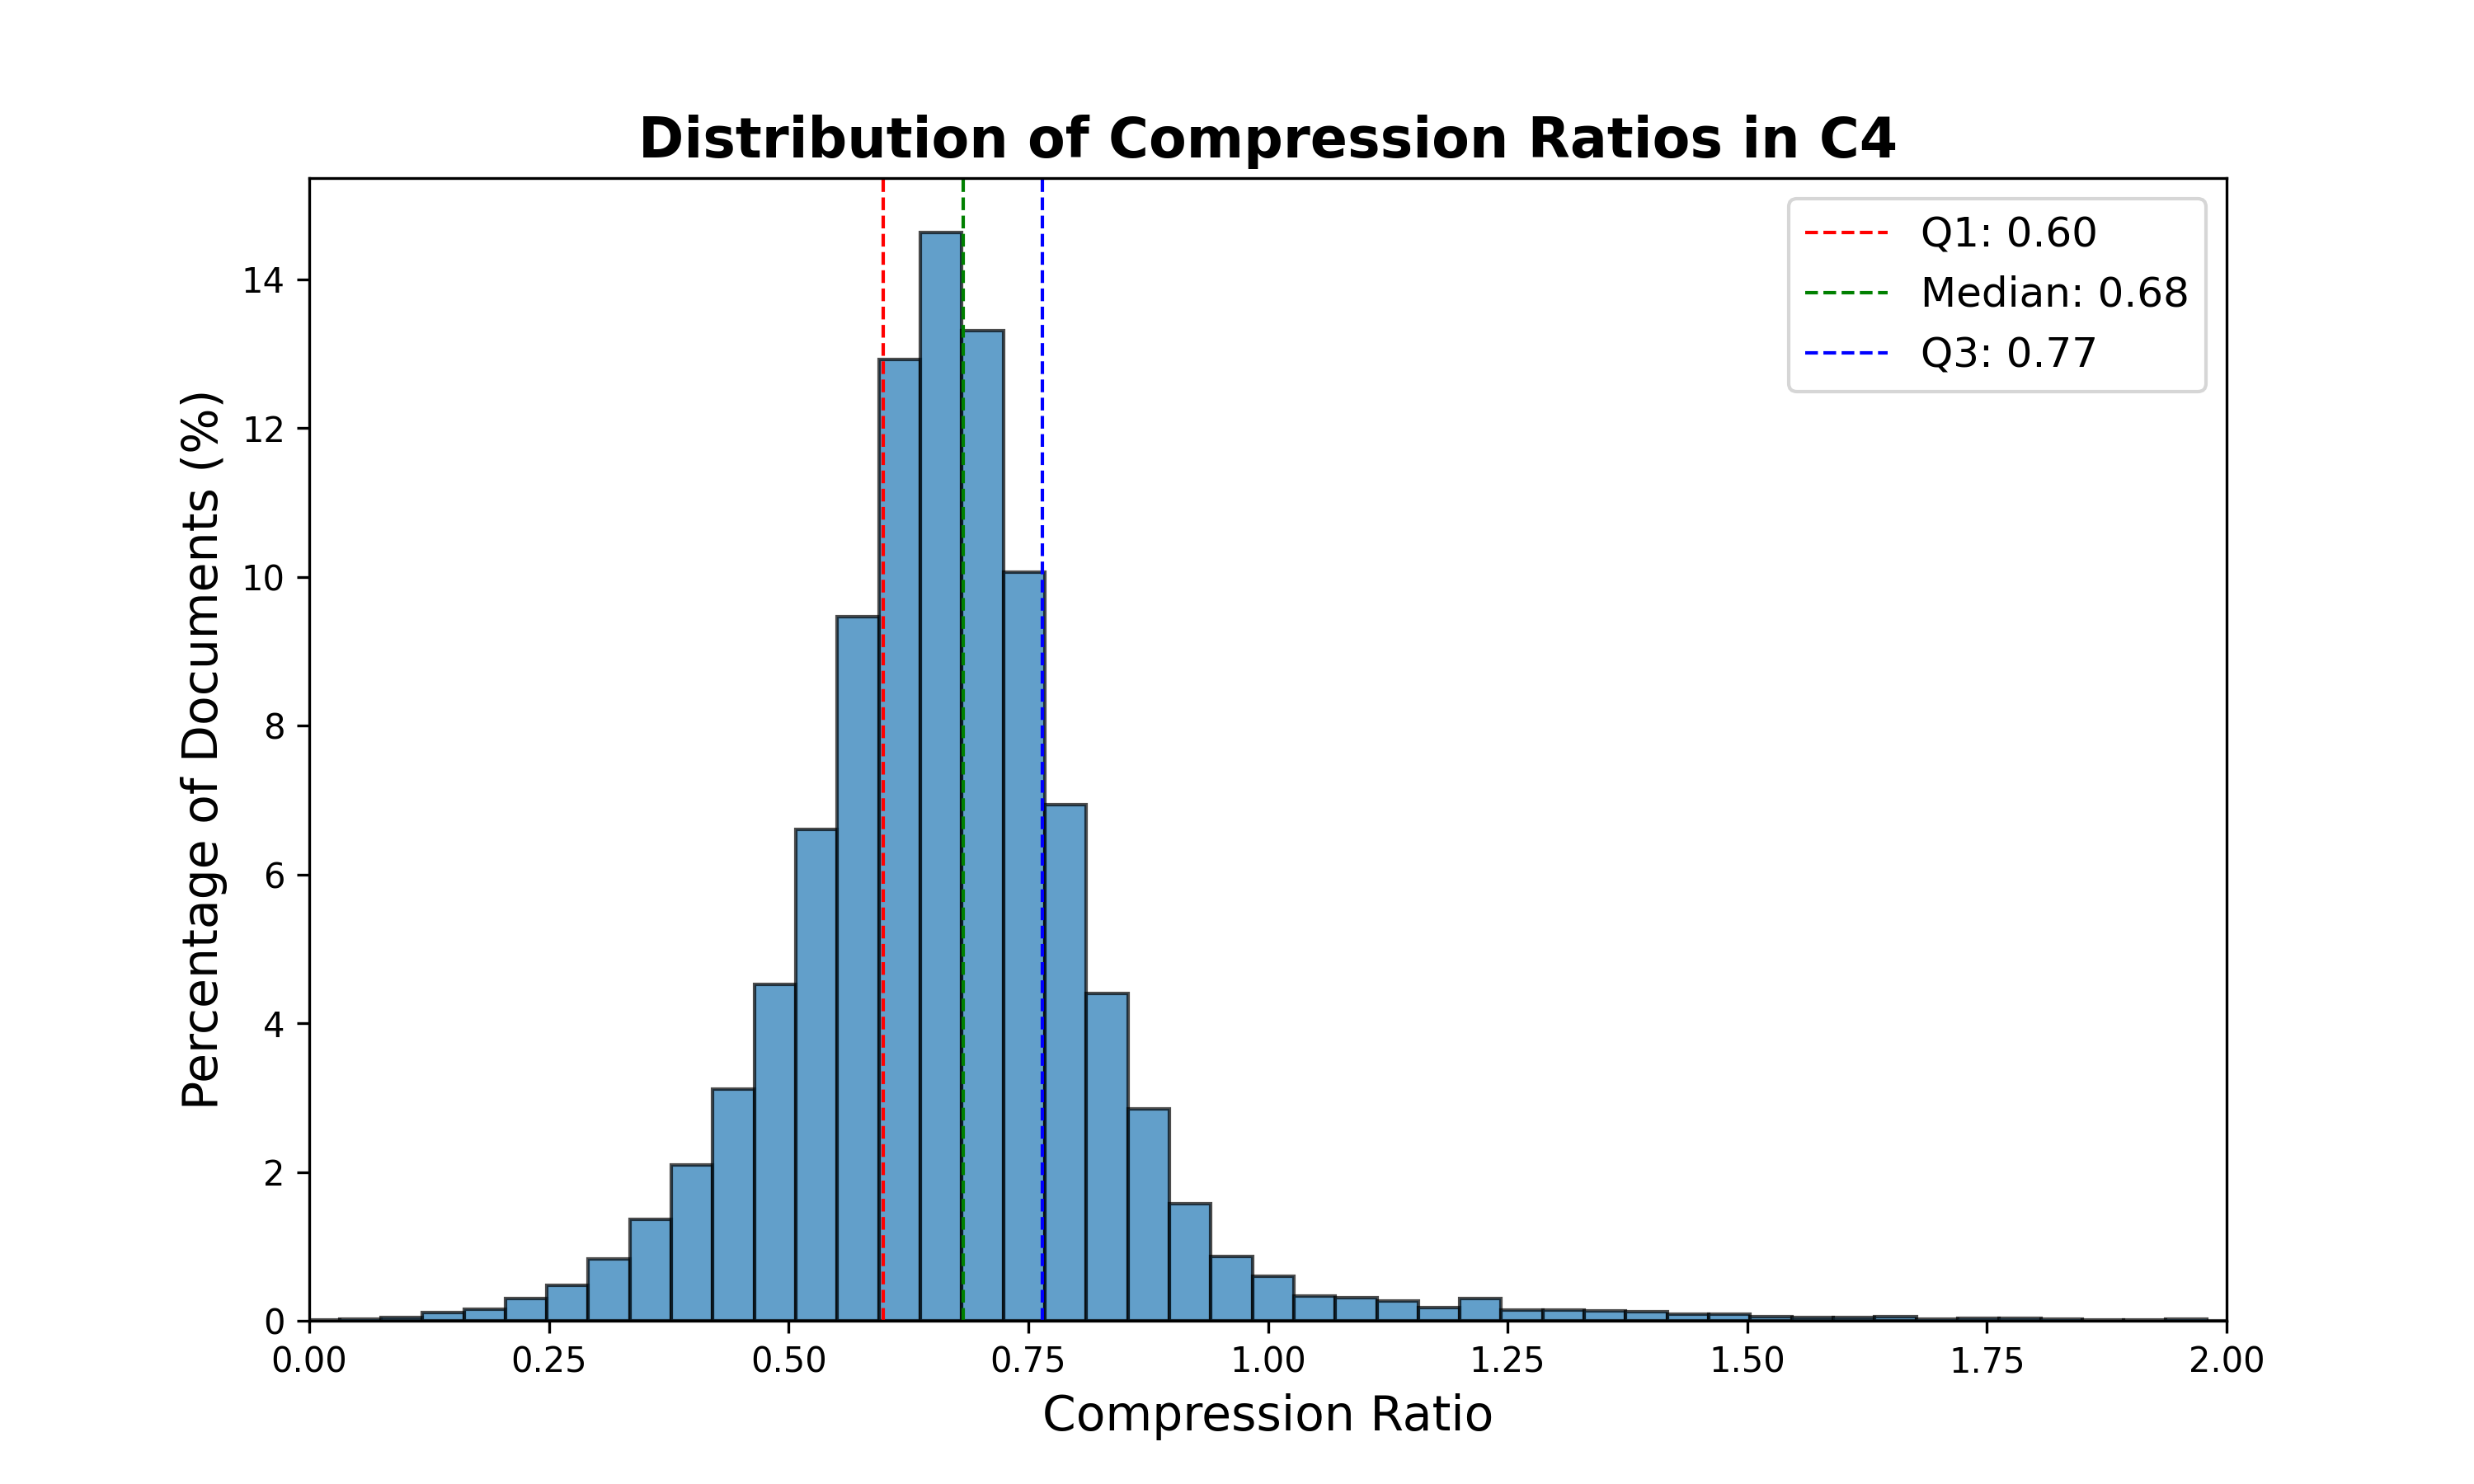
\includegraphics[width=0.49\textwidth]{fig3_cr_c4.png}\\[2pt]
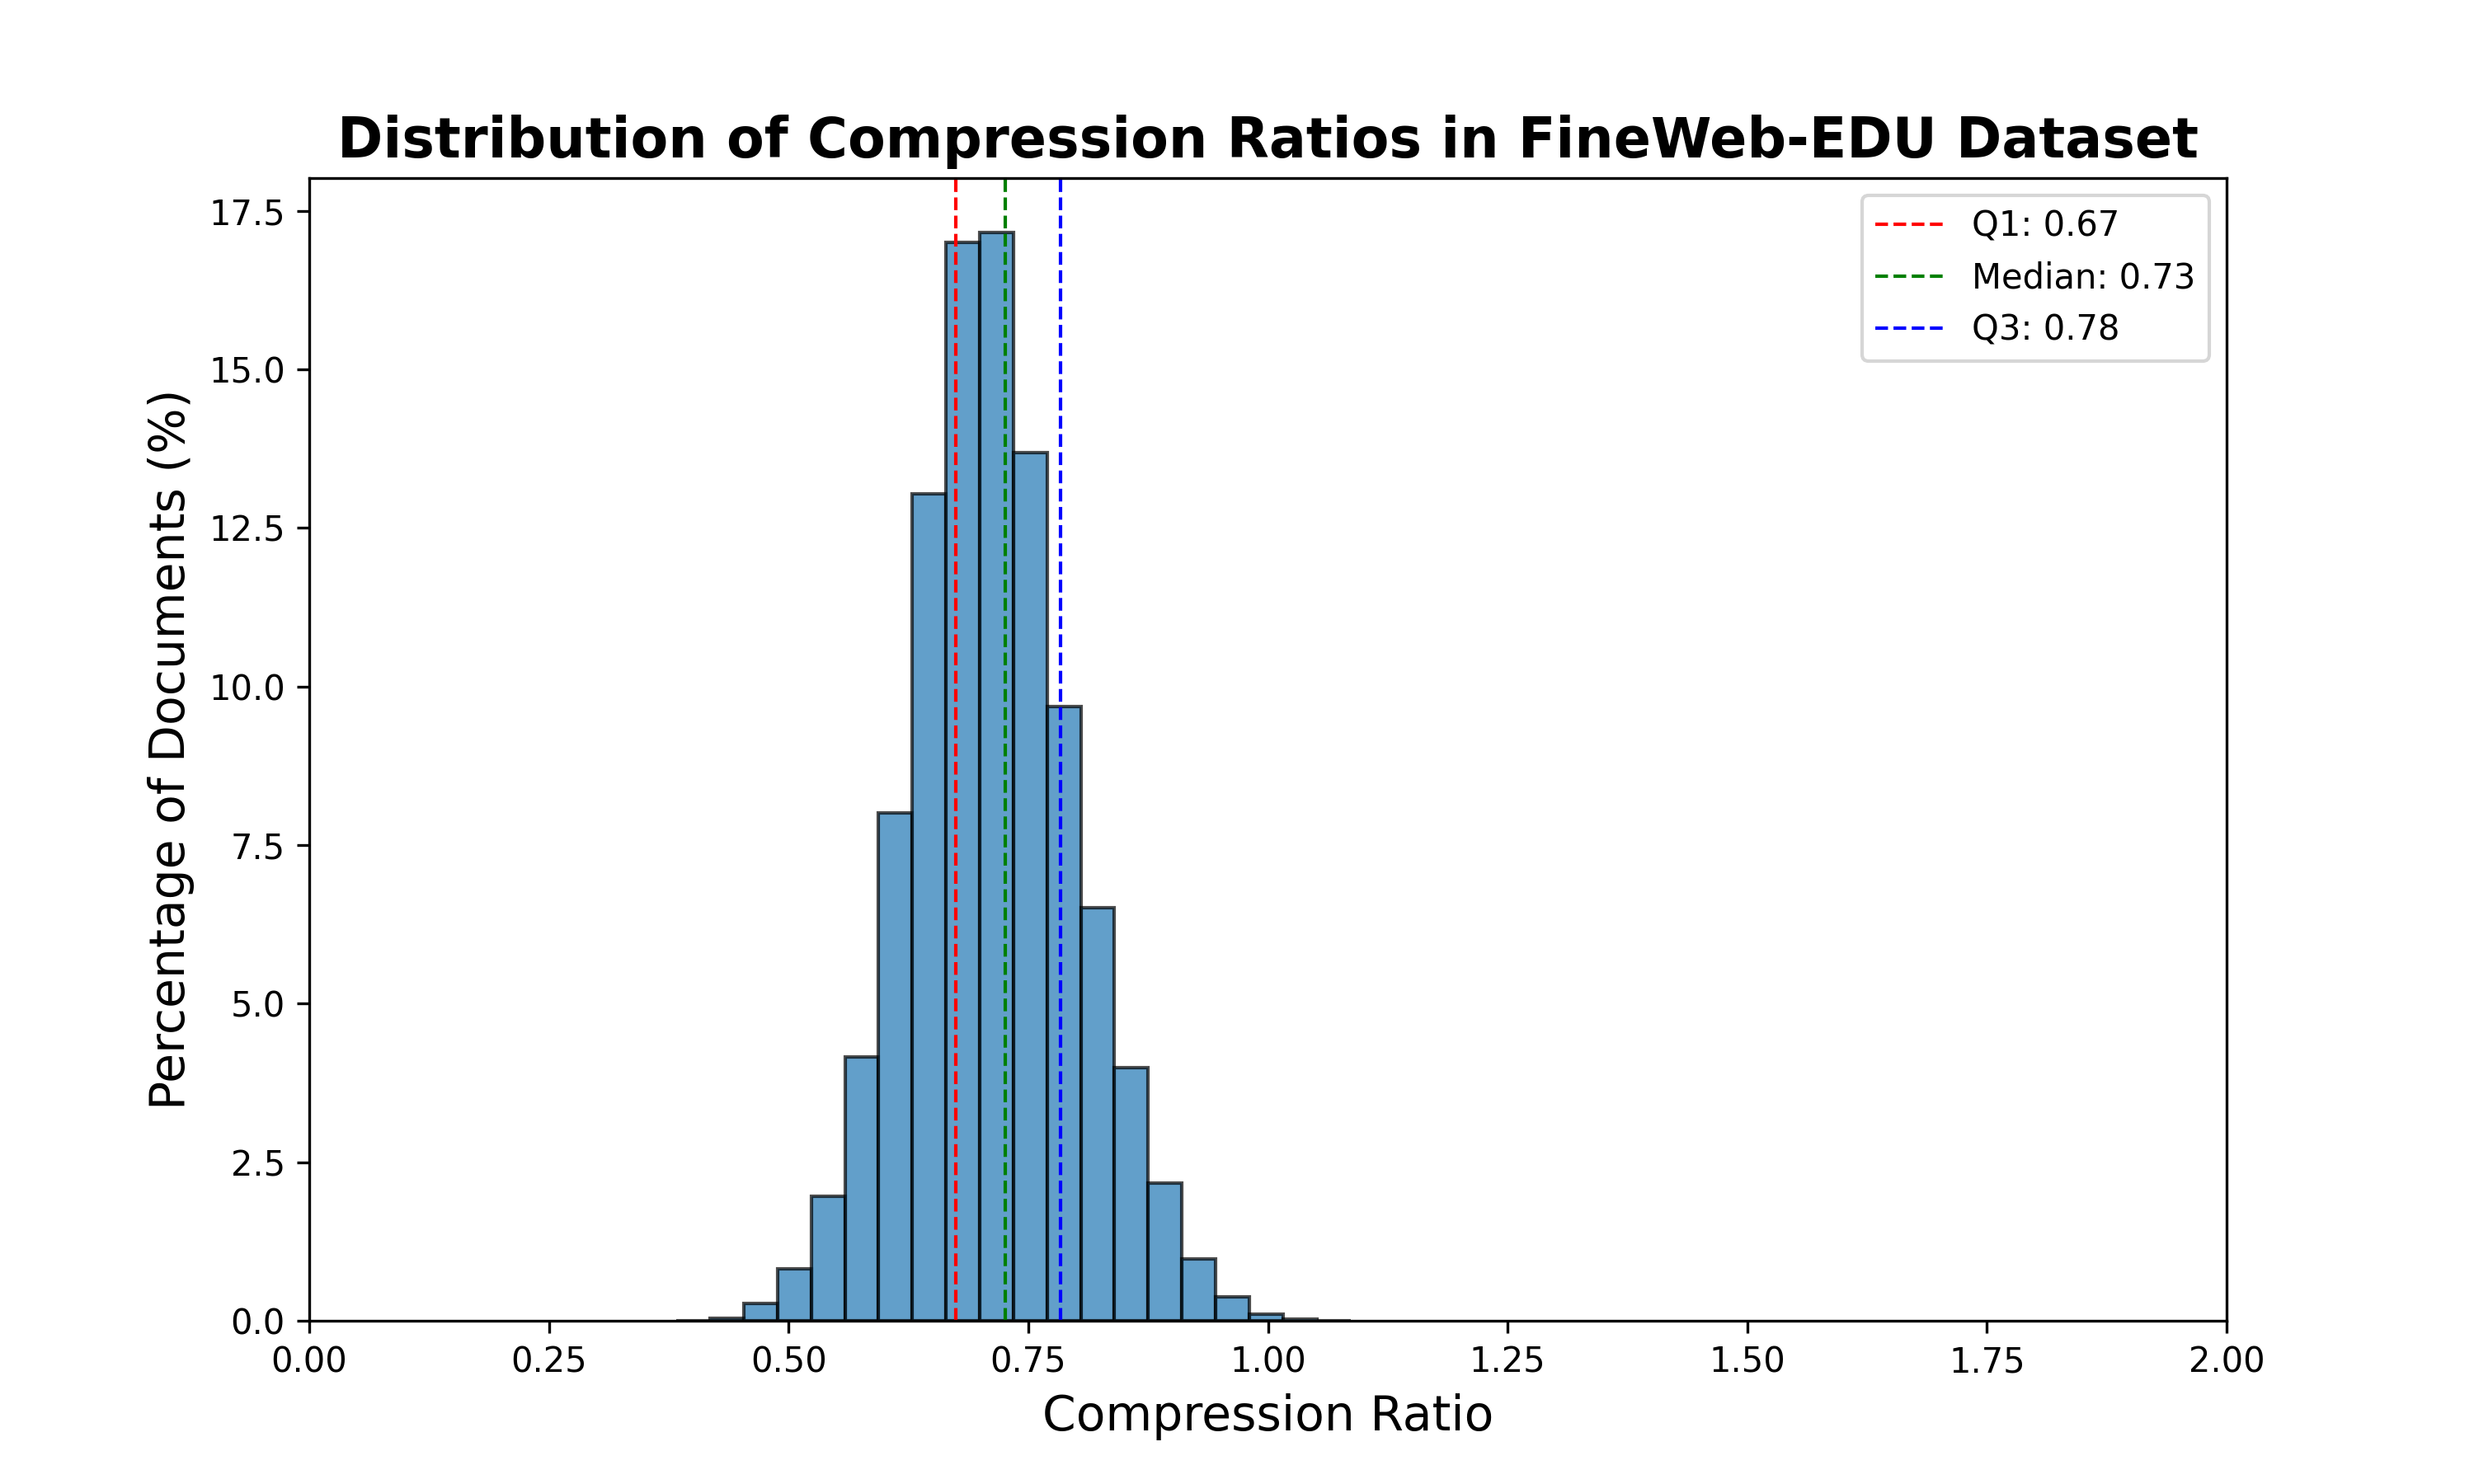
\includegraphics[width=0.49\textwidth]{fig3_cr_fineweb_edu.png}\hfill
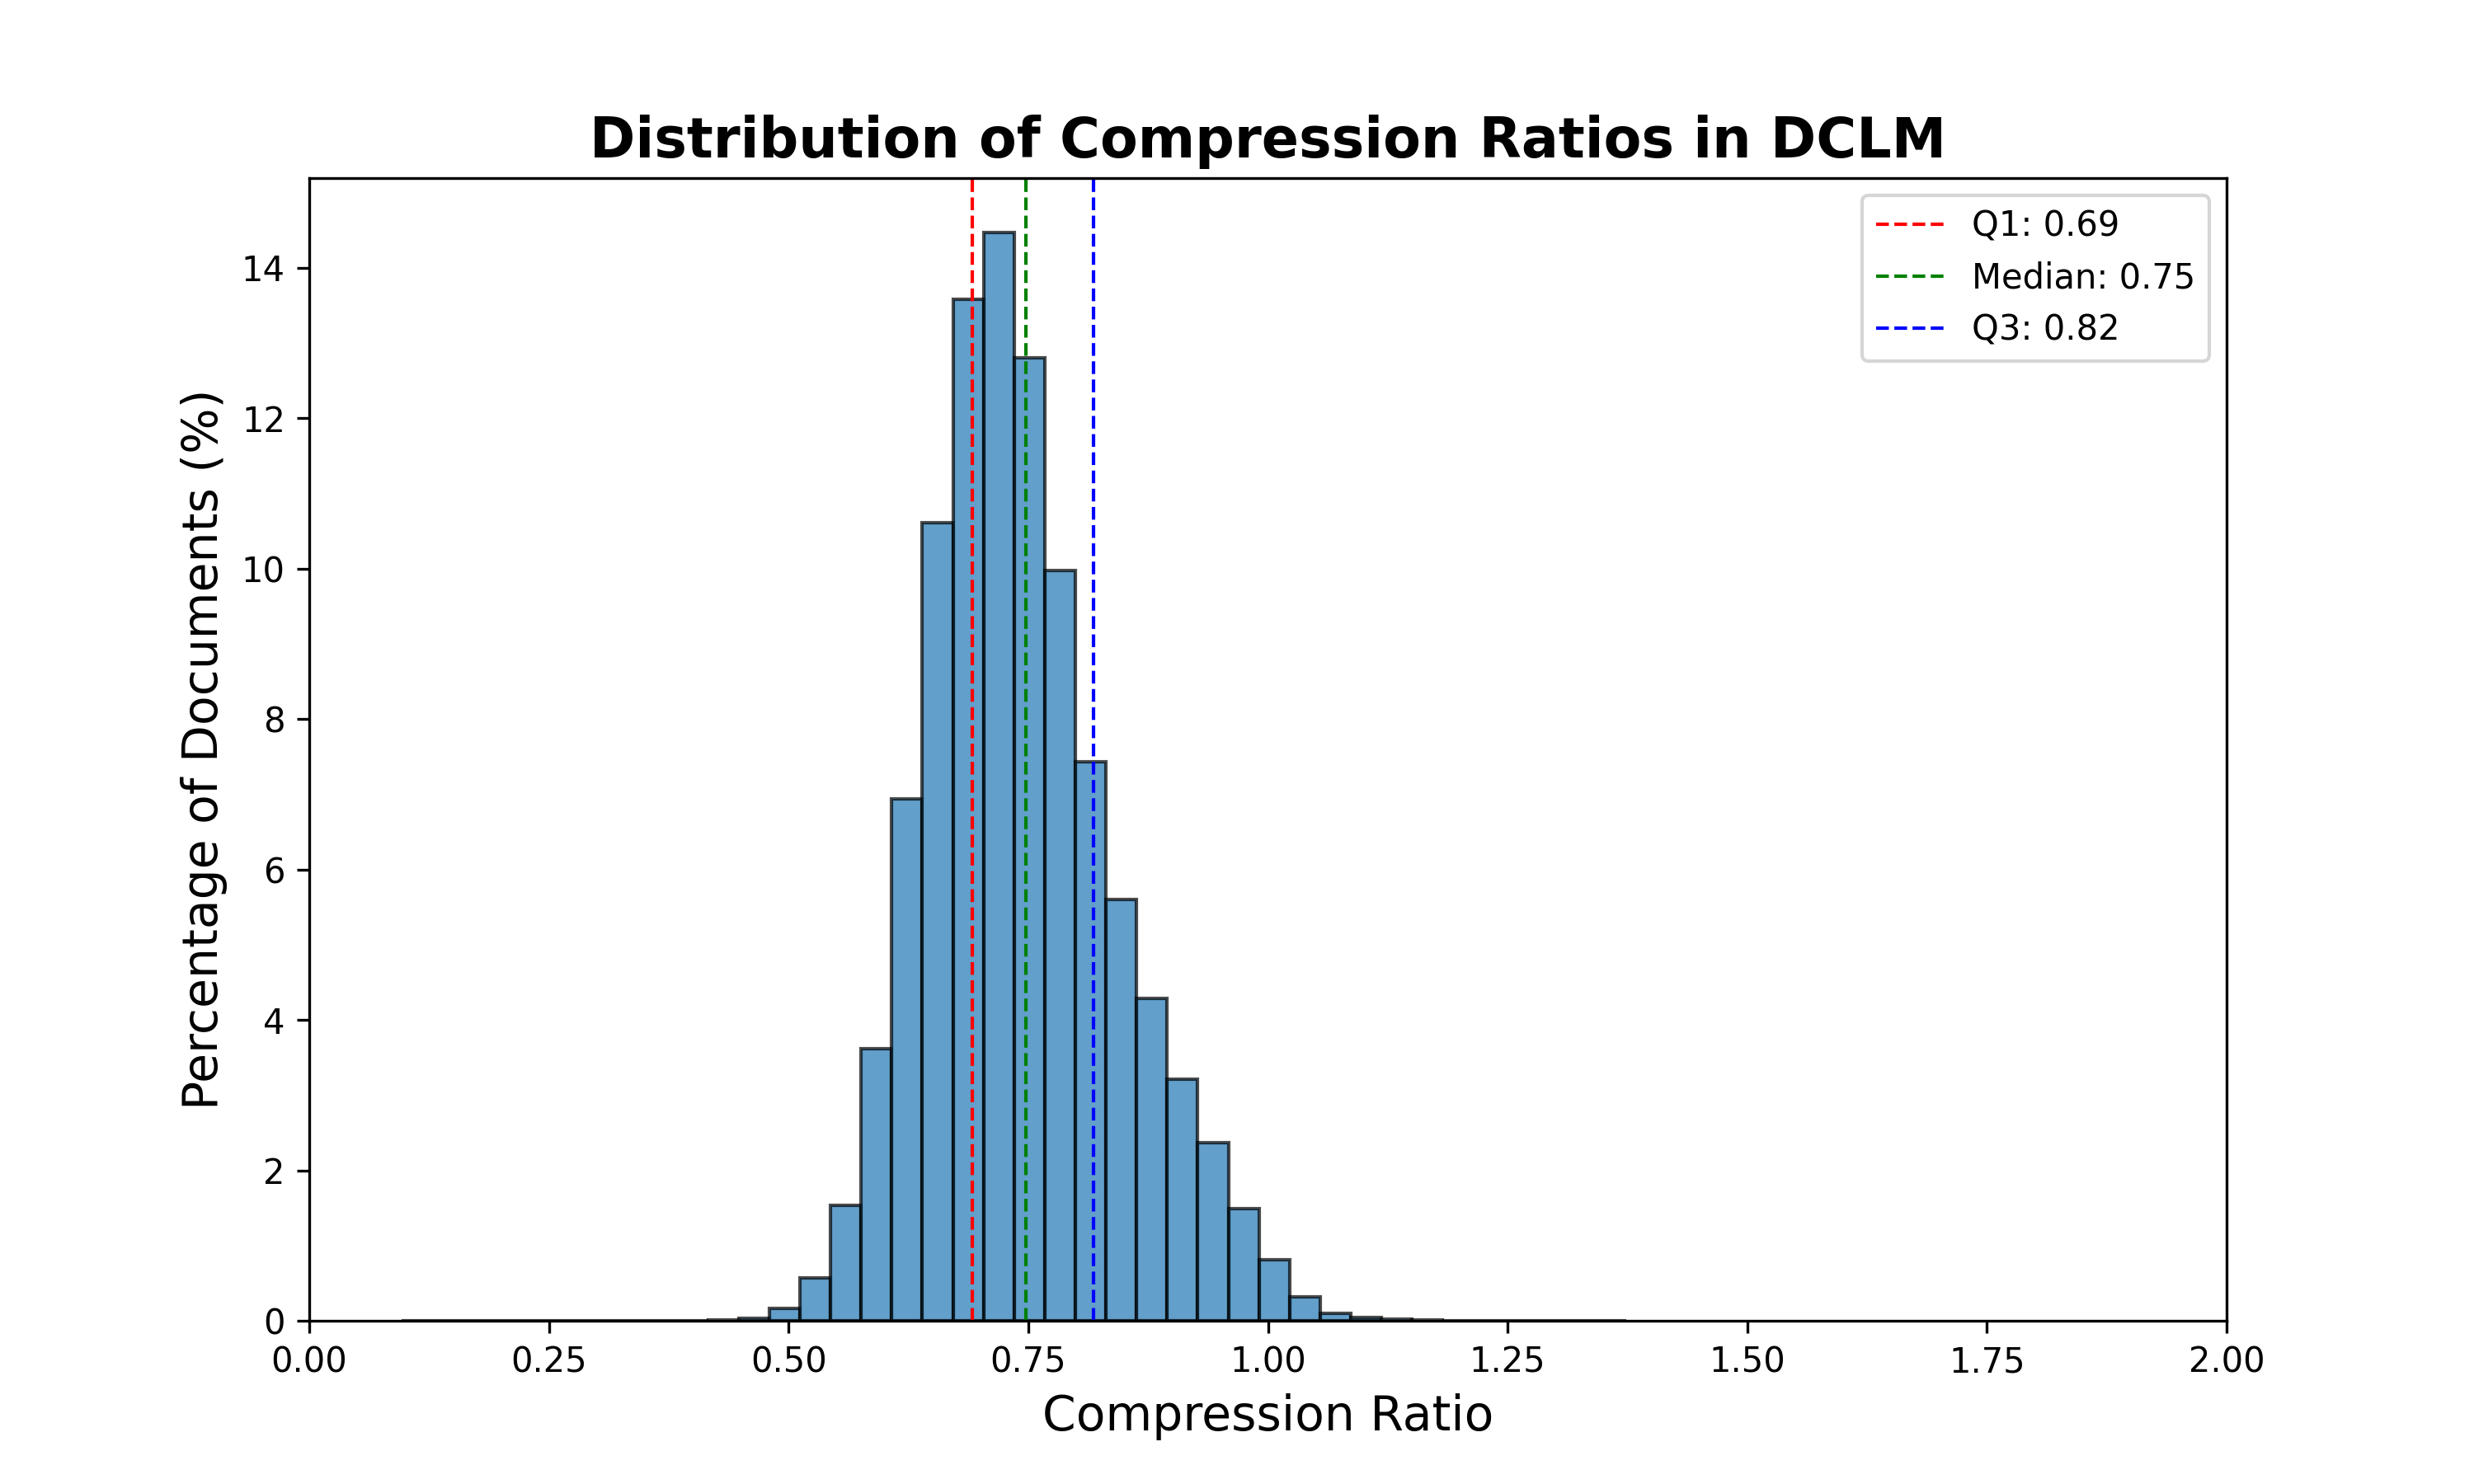
\includegraphics[width=0.49\textwidth]{fig3_cr_dclm.png}
\caption{\textbf{Compression ratio distributions across datasets.}
Each panel shows the LZ4 compression-ratio distribution of 1 million randomly sampled documents from the respective corpus.
\textbf{Top left:} Twitter (noisy, informal) skews high, with median CR $1.28$, reflecting structural noise and short, unstructured content.
\textbf{Top right:} C4 (minimally filtered) is broad with substantial tails.
\textbf{Bottom left:} FineWeb-EDU (heuristic plus classifier filtering) is more centralized.
\textbf{Bottom right:} DCLM (highly curated) peaks sharply near $0.75$.
As perceived dataset quality improves, the distribution narrows and centralizes.}
\label{fig:cr-distributions}
\end{figure}

Figure~\ref{fig:examples} shows examples of documents across different compression ratio bands.
Manual examination suggests that documents with compression ratios in a Goldilocks zone seem to correspond with higher quality text.
Low compression ratio documents frequently exhibit repetitive, templated text or keyword stuffing, while those with high compression ratios often feature noise, mixed-language content, or irregular formatting.
The intermediate range consistently contains structured, coherent, and informative text.

While these qualitative insights are compelling, we seek a more rigorous quantitative assessment.
To do this, we examine how compression ratio distributions change across datasets known to vary widely in quality.
Specifically, we ask: \emph{Do higher-quality datasets systematically exclude documents at the extremes of compression ratio distributions?}

To quantitatively investigate this, we analyze compression ratios over a random sample of 1 million documents from each of four corpora: C4, FineWeb-EDU, DCLM, and Twitter.
These datasets span a broad spectrum of curation strategies and observed downstream quality.
C4 is a minimally filtered Common Crawl dataset \citep{dodge2021documenting}; FineWeb-EDU applies heuristic and classifier-based filtering \citep{penedo2024fineweb}; DCLM undergoes model-based filtering \citep{li2024datacomp}; and Twitter consists of informal, noisy, and unstructured web content \citep{mohammad2018semeval, barbieri2018semeval}.
Figure~\ref{fig:cr-distributions} illustrates that as perceived dataset quality improves, compression ratio distributions become narrower and more centralized.
Lower-quality datasets like C4 have broader distributions with substantial tails, whereas higher-quality datasets such as DCLM exhibit tight, centralized distributions, effectively dropping documents with extreme compression ratios.

These correlational observations motivate a causal exploration: whether actively filtering documents based on compression ratio can concretely enhance downstream language model performance.
We explore this causal hypothesis in Section~\ref{sec:results}.

\subsection{Alignment with Existing Quality Signals}\label{sec:alignment}

\begin{figure}[t]
\centering
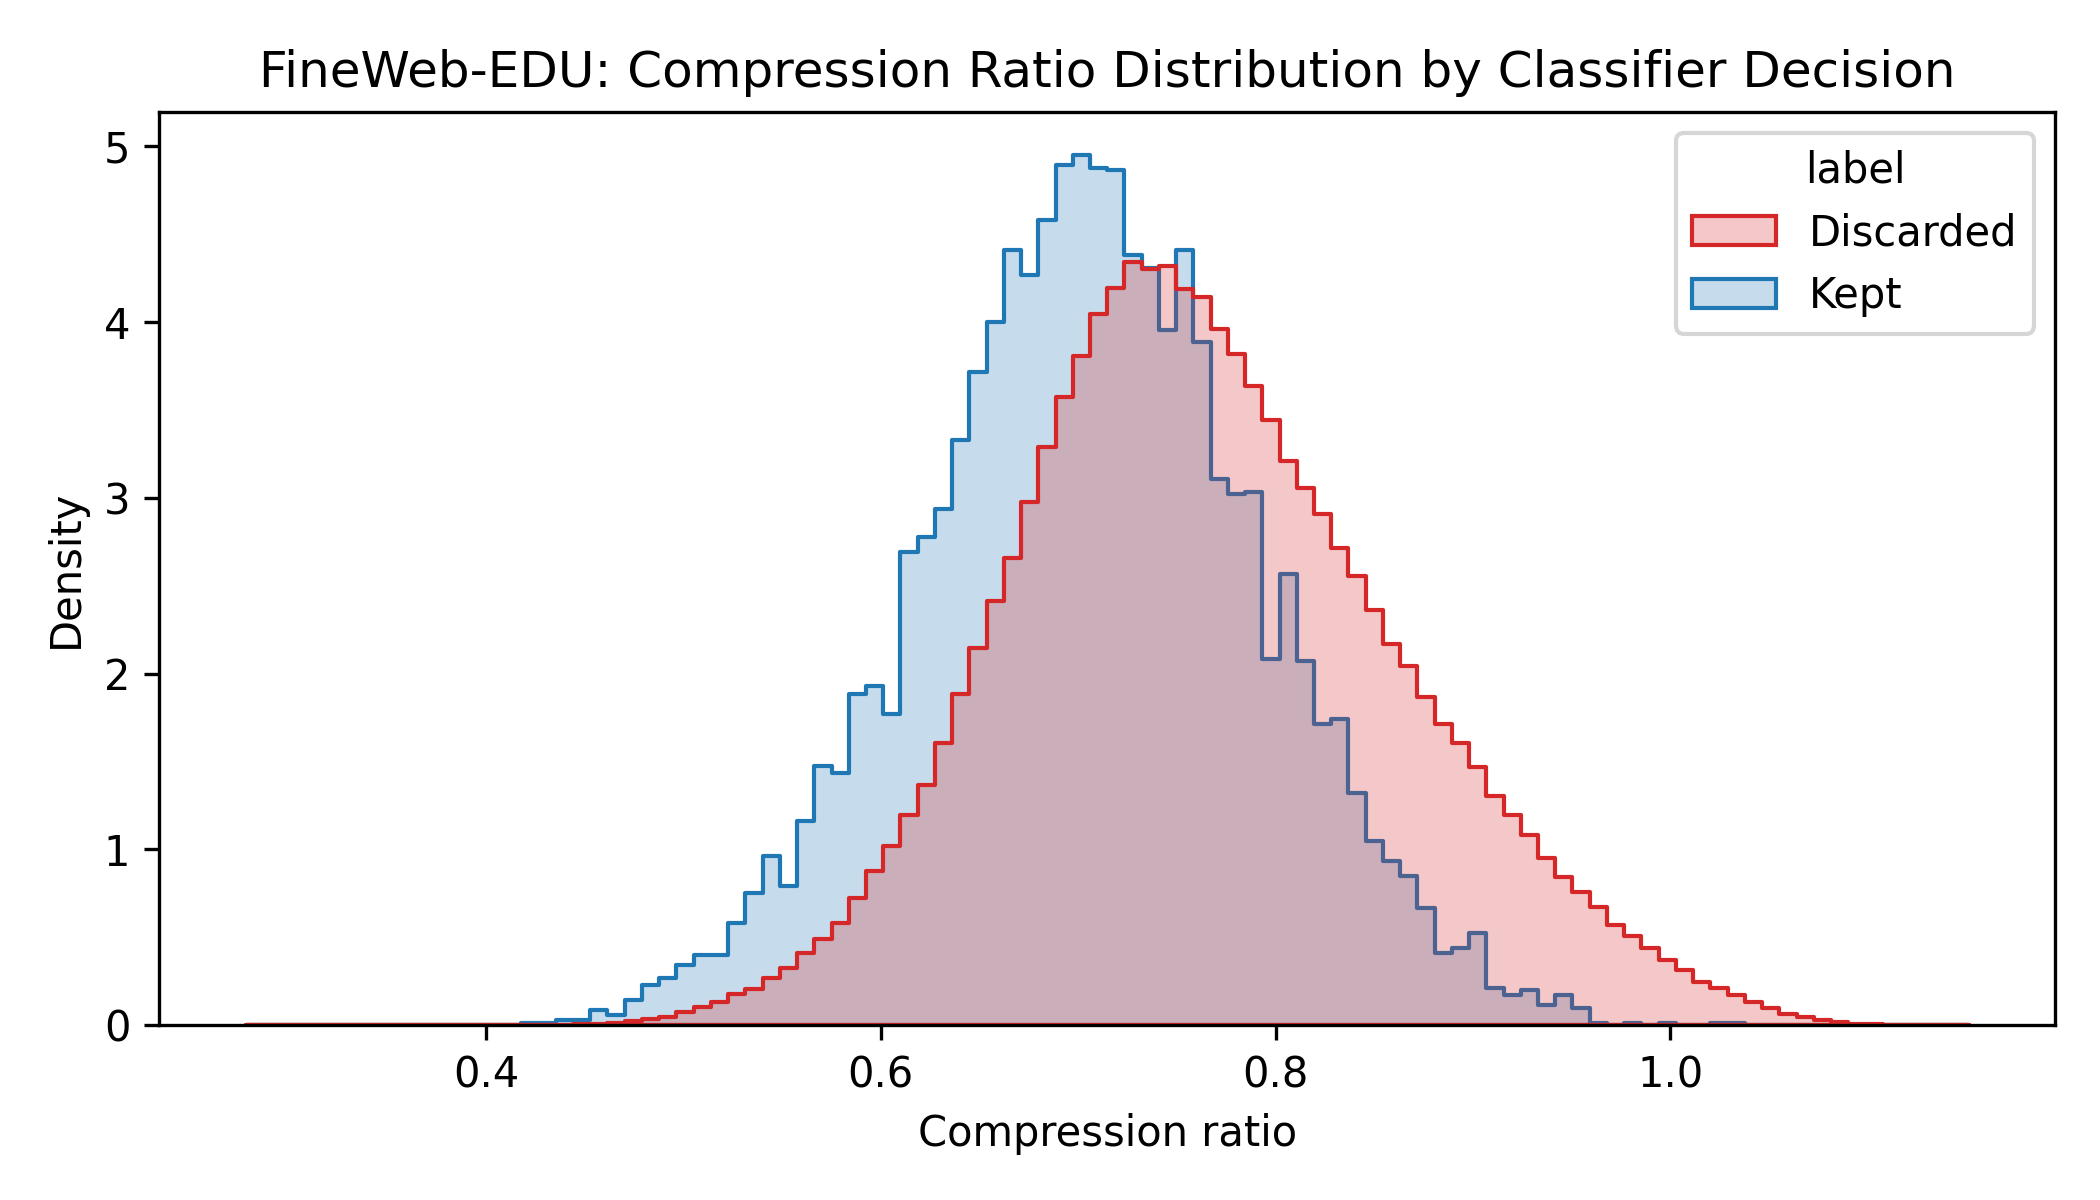
\includegraphics[width=0.72\textwidth]{fig4_fwedu_classifier_kde.png}
\caption{\textbf{Compression ratio mirrors many decisions made by the FineWeb-EDU quality classifier.}
We plot kernel-density estimates of the LZ4 compression ratio for one million randomly-sampled documents that the classifier \emph{keeps} (blue) versus \emph{discards} (red).
Lower ratios indicate text that is highly compressible (repetitive/boilerplate), whereas very high ratios often correspond to noisy or degenerate content.}
\label{fig:fwedu-kde}
\end{figure}

Figure~\ref{fig:fwedu-kde} provides evidence that compression ratio aligns closely with decisions made by the FineWeb-EDU quality classifier.
Documents accepted by this classifier predominantly occupy an intermediate compression ratio range (approximately 0.65--0.80), reflecting text that is sufficiently informative yet neither overly repetitive nor excessively noisy.
Conversely, documents discarded by the classifier display a broader compression ratio distribution, encompassing both highly repetitive (low compression) and noisy or irregular (high compression) extremes.

This alignment underscores compression ratio's utility as an intuitive, distributional proxy for textual quality, capturing much of the information implicitly used by more computationally demanding, model-based classifiers.
Nevertheless, the notable overlap between the ``kept'' and ``discarded'' distributions indicates inherent limitations of rigid thresholding strategies.
Many documents near the decision boundaries remain challenging to classify accurately via compression ratio alone.

% !TEX root = 00_dmlr_compel.tex
% New section for the DMLR version. Reviewers of an earlier draft judged the method
% "conceptually simple" and asked for deeper theoretical grounding; this section gives
% the Shannon / Kolmogorov / MDL reading of the Goldilocks band.
\section{Theoretical Grounding: Compression, Entropy, and Learnable Structure}\label{sec:theory}

A natural objection to \textsc{Compel} is that a single scalar seems too simple a statistic to carry information about data quality.
Information theory suggests otherwise: compression ratio estimates a document's entropy rate, and entropy rate separates the three regimes visible in Figure~\ref{fig:examples}.
This section makes that argument explicit.

\paragraph{Compression ratio estimates entropy rate.}
Shannon's source coding theorem states that no lossless code can use fewer expected bits per symbol than the entropy rate of the source, and that good codes approach this bound \citep{shannon1948mathematical}.
A practical compressor therefore acts as an entropy estimator: the length of $c(x)$ upper-bounds the information content of $x$ under the compressor's model class.
Shannon himself estimated the entropy of printed English this way, by measuring how far text could be predicted and hence compressed \citep{shannon1951prediction}.
In algorithmic terms, the ideal compressed length is the Kolmogorov complexity $K(x)$---the length of the shortest program that outputs $x$ \citep{kolmogorov1965three}.
$K$ is uncomputable, and real compressors are its standard computable surrogates \citep{li2008introduction}.
The same substitution underlies the Normalized Compression Distance \citep{cilibrasi2005clustering} and ZIP-FIT \citep{obbad2024zipfit}; $\mathrm{CR}(x)$ in Equation~\eqref{eq:cr} is simply the per-byte, normalized form of this surrogate.

\paragraph{Language modeling is compression.}
A language model with next-token distribution $p$ defines a lossless code that assigns $x$ a code length of $-\log_2 p(x)$ bits, so minimizing pretraining loss is exactly minimizing description length \citep{deletang2023language}.
Empirically, compression capacity tracks model capability \citep{huang2024compression}, and gzip compressibility predicts how scaling laws shift with data composition \citep{pandey2024gzip}.
Pretraining data value is therefore naturally measured in bits: a document is useful to the extent that it contains structure the model does not yet encode but can learn to encode.

\paragraph{Why both extremes are poor training data.}
The minimum description length (MDL) principle formalizes learning as two-part compression: a model part that captures regularity, and a residual part for what the model cannot explain \citep{rissanen1978modeling, grunwald2007minimum}.
The two tails of the compression-ratio distribution fail this decomposition in opposite ways.
When $\mathrm{CR}(x)$ is far below the band, the document's entropy rate is small: after a short prefix, additional tokens contribute almost no new bits (templated listings, keyword stuffing, boilerplate).
Gradient updates on such tokens repeat what the model has already absorbed, so we conjecture that they buy little generalization per FLOP.
When $\mathrm{CR}(x)$ is far above the band, the document is nearly incompressible for the LZ family, i.e., statistically close to random relative to that model class (hexadecimal tables, encoding artifacts, shuffled mixed-language spam).
A string that is algorithmically random admits no shorter description at all \citep{li2008introduction}; its loss is an irreducible noise floor, and capacity spent fitting it is capacity spent memorizing noise.

\paragraph{The interior band is where learnable structure lives.}
Between the extremes lies text with regularities that a weak universal compressor captures only partially: LZ4 exploits local repetition but not syntax, discourse, or semantics.
Precisely this residual structure is what a higher-capacity learner can still compress---that is, learn.
Well-edited human prose empirically concentrates in this regime (Figures~\ref{fig:cr-distributions} and~\ref{fig:fwedu-kde}), which explains why an interior compression-ratio band recovers much of the behavior of a trained quality classifier at a vanishing fraction of its cost.

\paragraph{Caveats.}
Two limits of this account deserve emphasis.
First, compression ratio is relative to the compressor: LZ4's window and parsing see local redundancy only, so the band $[0.65, 0.80]$ is a calibrated quantity, not a universal constant, and different compressors, scripts, or domains shift it (Section~\ref{sec:discussion}).
The bilingual example in Figure~\ref{fig:examples} compresses poorly partly for encoding reasons, not only for quality reasons.
Second, the account is first-order: it predicts that a useful interior band exists, not where its endpoints lie.
We therefore determine the endpoints empirically from high-quality reference corpora (Section~\ref{sec:method}).
In short, \textsc{Compel} operationalizes a classical idea: useful training text lives between the poles of redundancy and randomness---compressible enough to be structured, incompressible enough to be informative.

% !TEX root = 00_dmlr_compel.tex
\section{Compel: A Method for Improving Pretraining Data Quality}\label{sec:method}

\subsection{Desiderata}\label{sec:desiderata}

An effective data selection method for large-scale language model pretraining should satisfy the following criteria:
\begin{itemize}[leftmargin=1.35em,topsep=2pt,itemsep=1pt]
\item \textbf{Performance}: It should improve downstream accuracy or generalization relative to unfiltered or naively filtered data.
\item \textbf{Scalability}: It must operate efficiently over trillions of tokens.
\item \textbf{Simplicity}: The method should be easy to implement, interpret, and integrate into existing preprocessing pipelines.
\end{itemize}

\textsc{Compel} is designed with these criteria in mind.
It is an embedding-free, compression-based filtering method that improves data quality using a single, interpretable scalar: compression ratio.
It requires no training, inference, or human labels.

\subsection{Background: Compression Algorithms}\label{sec:background}

Lossless compression algorithms reduce file size by exploiting redundancy in the input.
In this work, we use LZ4, a fast, block-based compressor that employs LZ77-style sliding-window encoding.
LZ4 is streaming-compatible and operates over raw byte strings, making it ideal for large-scale filtering pipelines.
Unlike perplexity scores or embedding distances, compression operates without tokenization, external supervision, or model inference.

\subsection{Filtering Criteria}\label{sec:filtering}

Based on empirical observations from Section~\ref{sec:cr-signal}, we define a quality band of compression ratios: $\tau_{\min} = 0.65$ and $\tau_{\max} = 0.80$.
Let $\mathcal{D} = \{x_1, x_2, \dots, x_N\}$ be a collection of documents in a pretraining corpus.
Documents with $\mathrm{CR}(x) \in [\tau_{\min}, \tau_{\max}]$ are retained.
Those falling outside this range are discarded.
These threshold values were selected based on the inter-quartile ranges observed in high-quality datasets like DCLM and FineWeb-EDU, where well-structured, information-dense documents tend to fall within this band.
This provides a simple, domain-agnostic filter that effectively removes both overly redundant and noisy examples.
Section~\ref{sec:theory} gives the information-theoretic reading of this band.

\subsection{Efficiency}\label{sec:efficiency}

\textsc{Compel} is highly efficient and trivially parallelizable.
On a machine with 500 CPUs, the filter processes over 40{,}000 documents per second using LZ4 compression---an order of magnitude faster than typical perplexity- or classifier-based quality filters.

% !TEX root = 00_dmlr_compel.tex
\section{Experiments}\label{sec:experiments}

\subsection{Pretraining Corpora}\label{sec:corpora}

We evaluate \textsc{Compel} on three widely-used corpora for language model pretraining:
\begin{itemize}[leftmargin=1.35em,topsep=2pt,itemsep=1pt]
\item \textbf{FineWeb} \citep{penedo2024fineweb}: A 15-trillion-token web crawl filtered with domain heuristics and safety constraints.
\item \textbf{FineWeb-EDU} \citep{penedo2024fineweb}: A 1.3-trillion-token educational subset extracted using a synthetic LLM classifier trained on LLaMA 3 70B-Instruct annotations.
\item \textbf{DCLM} \citep{li2024datacomp}: A 4-trillion-token corpus derived from Common Crawl, curated to support high-accuracy model training with limited compute.
\end{itemize}

For each corpus, we construct a \emph{\textsc{Compel}-filtered} variant by removing documents whose LZ4 compression ratio falls outside the calibrated range:
\begin{equation*}
\tau_{\min} = 0.65, \qquad \tau_{\max} = 0.80.
\end{equation*}
Compression is applied to raw byte-level representations using a single pass over the dataset.
Filtering is performed prior to tokenization and shuffling.

\subsection{Model Configurations}\label{sec:models}

For each \textsc{Compel}-filtered variant, we train two decoder-only Transformer models based on the LLaMA architecture \citep{touvron2023llama} with rotary position embeddings and grouped-query attention.
The \textbf{1.4B model} has 16 layers, a hidden size of 2048, intermediate size of 7168, 16 attention heads, and 8 key/value heads.
The \textbf{8B model} consists of 32 layers, a hidden size of 4096, intermediate size of 14336, 32 attention heads, and 8 key/value heads.
Both models are configured with a maximum sequence length of 4096.
These values were selected based on standard configurations shown to perform well at this scale in prior open-source models.
The 8B model follows the LLaMA 3 hyperparameters \citep{touvron2023llama}, which are tuned for stability and efficiency at high model capacity.
All models are trained from scratch without weight reuse or initialization from pretrained checkpoints.

\subsection{Training Protocol}\label{sec:training}

The \textbf{1.4B model} is trained for 10{,}000 steps using a batch size of 1024 and sequence length of 4096, totaling 42 billion tokens.
The \textbf{8B model} is trained for 40{,}000 steps under the same sequence length and batch size, totaling 167 billion tokens.
Training is performed on TPU v4-128 pods.

We use AdamW optimization for all models.
The 1.4B model uses a learning rate of $3 \times 10^{-4}$ with weight decay of 0.1.
% TODO(internal-review): 2e-3 for the 8B looks high vs LLaMA-3's ~3e-4; this value is transcribed
% from the Dec-2025 review PDF — confirm the actual run config with Elyas before camera-ready.
The 8B model follows the LLaMA 3 hyperparameters: a learning rate of $2 \times 10^{-3}$, weight decay 0.05, and 5000 warmup steps.
All models are trained with cosine decay schedules and dropout rate of 0.1.

\subsection{Evaluation Suite}\label{sec:evaluation}

We evaluate each model using the standardized \texttt{lm-eval-harness} framework \citep{biderman2024lessons}, following zero-shot protocols on a diverse set of 13 natural language processing benchmarks:
\begin{itemize}[leftmargin=1.35em,topsep=2pt,itemsep=1pt]
\item \textbf{Commonsense and Reasoning:} COPA \citep{roemmele2011choice}, CommonsenseQA \citep{talmor2018commonsenseqa}, PIQA \citep{bisk2020piqa}, ARC (Easy/Challenge) \citep{clark2018think}, AGIEval LSAT-AR \citep{zhong2023agieval}
\item \textbf{Reading Comprehension:} BoolQ \citep{clark2019boolq}, OpenBookQA \citep{mihaylov2018suit}, WinoGrande \citep{sakaguchi2021winogrande}, WSC273 \citep{levesque2012winograd}, LAMBADA \citep{paperno2016lambada}
\item \textbf{Multichoice QA:} HellaSwag (0-shot, 10-shot) \citep{zellers2019hellaswag}
\end{itemize}

\paragraph{Metrics.}
We report task-standard metrics for each dataset, primarily multiple-choice question-answering accuracy.
We aggregate results using unweighted macro-average accuracy over all tasks.

% !TEX root = 00_dmlr_compel.tex
\section{Results}\label{sec:results}

We evaluate \textsc{Compel} across three widely-used, large-scale pretraining datasets---FineWeb, FineWeb-EDU, and DCLM---using two LLaMA-style model scales: 1.4 billion (1.4B) and 8 billion (8B) parameters.
We measure model performance using macro-average accuracy across a suite of 13 diverse downstream benchmarks (see Section~\ref{sec:evaluation}).
The detailed benchmark results are summarized in Table~\ref{tab:results-1p4b}, with key findings discussed below.

\subsection{Impact of Compression-Based Filtering at 1.4B Scale}\label{sec:results-1p4b}

\begin{table}[t]
\centering
\caption{\textbf{Results for 1.4B-parameter models across datasets.}
\textsc{Compel} improves on 9 out of 13 benchmarks for FineWeb, 9 out of 13 for FineWeb-EDU, and 11 out of 13 for DCLM.
Green marks improvements over the corresponding unfiltered baseline; red marks regressions.}
\label{tab:results-1p4b}
\small
\setlength{\tabcolsep}{4.5pt}
\begin{tabular}{lcccccc}
\toprule
 & \multicolumn{2}{c}{FineWeb} & \multicolumn{2}{c}{FineWeb-EDU} & \multicolumn{2}{c}{DCLM} \\
\cmidrule(lr){2-3}\cmidrule(lr){4-5}\cmidrule(lr){6-7}
Benchmark & Base & +\textsc{Compel} & Base & +\textsc{Compel} & Base & +\textsc{Compel} \\
\midrule
WSC273             & 0.571 & \imp{0.604} & 0.571 & \reg{0.550} & 0.630 & \imp{0.637} \\
Winogrande         & 0.528 & \imp{0.534} & 0.532 & \reg{0.525} & 0.528 & \imp{0.539} \\
PIQA               & 0.708 & \imp{0.712} & 0.687 & \imp{0.702} & 0.705 & \imp{0.710} \\
OpenBookQA         & 0.196 & \reg{0.192} & 0.244 & \imp{0.258} & 0.222 & \imp{0.230} \\
LAMBADA            & 0.369 & \imp{0.379} & 0.337 & \imp{0.339} & 0.499 & \imp{0.501} \\
HellaSwag (10-shot)& 0.362 & \imp{0.365} & 0.365 & \reg{0.364} & 0.371 & \imp{0.378} \\
HellaSwag (0-shot) & 0.365 & \imp{0.369} & 0.378 & \imp{0.384} & 0.375 & \imp{0.379} \\
COPA               & 0.630 & \imp{0.730} & 0.690 & \imp{0.730} & 0.690 & \imp{0.710} \\
CommonsenseQA      & 0.201 & \reg{0.188} & 0.216 & \reg{0.197} & 0.199 & \imp{0.207} \\
BoolQ              & 0.591 & \imp{0.593} & 0.571 & \imp{0.606} & 0.507 & \reg{0.462} \\
ARC-Easy           & 0.537 & \reg{0.536} & 0.623 & \imp{0.634} & 0.609 & \imp{0.614} \\
ARC-Challenge      & 0.230 & \reg{0.218} & 0.282 & \imp{0.296} & 0.276 & \reg{0.265} \\
AGIEval LSAT-AR    & 0.230 & \imp{0.239} & 0.248 & \imp{0.257} & 0.217 & \imp{0.222} \\
\midrule
\textbf{Macro avg.}& 0.424 & \imp{0.435} & 0.442 & \imp{0.449} & 0.466 & \imp{0.470} \\
\bottomrule
\end{tabular}
\end{table}

\paragraph{FineWeb.}
As shown in Table~\ref{tab:results-1p4b}, \textsc{Compel}-filtered models improve accuracy on 9 out of 13 tasks compared to the heavily-filtered FineWeb baseline, yielding a notable macro-average accuracy increase of 1.1 points (from 42.4\% to 43.5\%).
The largest improvements occur in commonsense reasoning benchmarks, notably COPA (+10\%) and WSC273 (+3.3\%), suggesting that removing documents outside the calibrated compression ratio range effectively eliminates subtle forms of noise, enhancing models' reasoning capabilities.

\paragraph{FineWeb-EDU.}
Even though FineWeb-EDU is already filtered via strong classifier-based heuristics, \textsc{Compel} further enhances model performance.
As Table~\ref{tab:results-1p4b} indicates, \textsc{Compel} filtering leads to improved accuracy on 9 of 13 tasks, resulting in a 0.7-point increase in macro-average accuracy (from 44.2\% to 44.9\%).
Notable gains are observed on COPA (+4\%) and BoolQ (+3.5\%).

\paragraph{DCLM.}
DCLM represents the current gold standard in dataset quality.
Nevertheless, Table~\ref{tab:results-1p4b} reveals that \textsc{Compel} still offers improvements on 11 of 13 tasks, yielding a 0.4-point increase in macro-average accuracy (from 46.6\% to 47.0\%).

\subsection{Effectiveness of \textsc{Compel} at Larger Model Scale (8B)}\label{sec:results-8b}

Our 8B experiments demonstrate that \textsc{Compel}'s effectiveness persists at scale: it improves both macro and micro average accuracy despite the increased capacity and learning dynamics of larger models.
This suggests that \textsc{Compel}'s benefits are not confined to small or medium-scale settings.
Instead, compression-based filtering enhances training efficiency even when models have greater capacity to absorb noise, indicating that the quality improvements it introduces are fundamental rather than compensatory.
As model sizes continue to grow, such lightweight filters can play an increasingly important role in optimizing compute budgets while preserving or improving performance.

Task-level results reveal notable improvements in tasks such as BoolQ (+5.5\%) and CommonsenseQA (+2.6\%), despite minor regressions on ARC-Challenge ($-$2.4\%) and WSC273 ($-$1.1\%).
These results highlight that \textsc{Compel} filtering scales effectively with increased model size, preserving or enhancing model capabilities and improving data efficiency without added computational complexity.

\begin{table}[t]
\centering
\caption{\textbf{Results on 8B models trained on FineWeb.}
\textsc{Compel} preserves or slightly improves downstream accuracy (macro average $0.570 \rightarrow 0.572$, micro average $0.587 \rightarrow 0.593$).}
\label{tab:results-8b}
\small
\begin{tabular}{lcc}
\toprule
Benchmark & FineWeb & FineWeb + \textsc{Compel} \\
\midrule
WSC273             & 0.809 & \reg{0.798} \\
Winogrande         & 0.682 & \reg{0.679} \\
PIQA               & 0.793 & \reg{0.791} \\
OpenBookQA         & 0.310 & 0.310 \\
LAMBADA            & 0.638 & \imp{0.648} \\
HellaSwag (10-shot)& 0.556 & \imp{0.561} \\
HellaSwag (0-shot) & 0.562 & 0.562 \\
COPA               & 0.860 & \reg{0.850} \\
CommonsenseQA      & 0.189 & \imp{0.215} \\
BoolQ              & 0.683 & \imp{0.738} \\
ARC-Easy           & 0.705 & \imp{0.732} \\
ARC-Challenge      & 0.396 & \reg{0.372} \\
AGIEval LSAT-AR    & 0.204 & \imp{0.213} \\
\midrule
\textbf{Macro avg.} & 0.570 & \imp{0.572} \\
\textbf{Micro avg.} & 0.587 & \imp{0.593} \\
\bottomrule
\end{tabular}
\end{table}

% !TEX root = 00_dmlr_compel.tex
\section{Compel Qualitatively Selects Higher Quality Text}\label{sec:qualitative}

To better understand the kinds of documents filtered by compression ratio, we visualize examples from each compression band: low ($<0.65$), \textsc{Compel}-kept ($0.65$--$0.80$), and high ($>0.80$).
We display the beginning lines of real web documents from each region in Figure~\ref{fig:examples}.

\begin{figure}[t]
\centering
\small
\begin{tabular}{p{0.30\textwidth} p{0.30\textwidth} p{0.30\textwidth}}
\toprule
$\mathrm{CR} < 0.65$ & $0.65 \le \mathrm{CR} \le 0.80$ & $\mathrm{CR} > 0.80$ \\
\midrule
\emph{Asus Laptop Virus Removal Asus Repair Service Area: Asus Laptop Virus Removal Toronto, Laptop Repair GTA, Laptop Repair Thornhill, Laptop Repair Richmond Hill, Laptop Repair Markham, Laptop Repair Vaughan, Laptop Repair Toronto, Laptop Repair Scarborough, Laptop Repair Newmarket, Laptop Repair Mississauga...}
&
\emph{This project is solving the Asteroid Watchers challenge. AROs are essentially created by combining a telescope with a smartphone. If the telescope has drive motors controllable via a standard // protocol, it is commanded by the SkyWatch app on the phone. Telescopes without motors need an Arduino-driven stepper setup. We plan to publish a...}
&
\emph{\begin{CJK}{UTF8}{gbsn}根香港法律,不得在程中,向未成年人售或供令人醺醉的酒。\end{CJK} Under the law of Hong Kong, intoxicating liquor must not be sold or supplied to a minor in the course of business. Enjoy FREE DELIVERY for orders HK\$1500 (net) or more, otherwise a delivery charge may apply. Hotline: +852 9063 3222 visa visa verified master master secure paypal...} \\
\bottomrule
\end{tabular}
\caption{\textbf{Beginning characters of representative examples} excluded for low compression ratio (left), kept by \textsc{Compel} (middle), and excluded for high compression ratio (right).
\textsc{Compel} retains the informative mid-range while filtering boilerplate or noisy text.}
\label{fig:examples}
\end{figure}

The low-compression examples are dominated by boilerplate keyword stuffing and templated text (e.g., location-specific service listings repeated verbatim).
High-compression examples tend to be noisy, short, or include artifacts like mixed-language metadata or hexadecimal tables.
In contrast, documents retained by \textsc{Compel} exhibit higher information density and structural coherence---typically consisting of fluent, formal descriptions, educational explanations, or open-source project write-ups.

Qualitatively, \textsc{Compel} effectively discards content at both ends of the redundancy--entropy spectrum, keeping the center band where well-edited, human-authored text lies.
This confirms the value of compression ratio as a simple yet powerful signal for improving pretraining data quality.

% !TEX root = 00_dmlr_compel.tex
\section{Discussion and Limitations}\label{sec:discussion}

\textsc{Compel} was designed to address a fundamental challenge in large-scale language model training: identifying and filtering high-quality data from internet-scale corpora without incurring the cost of large models, supervision, or inference.
While individual gains from \textsc{Compel} filtering are modest (+0.4--1.1 points), our results demonstrate that these gains are consistent across datasets and model sizes, achieved with negligible computational overhead.

Prior work shows that small, reproducible accuracy improvements can have outsize benefits at scale \citep{marion2023less, ankner2024perplexed, tirumala2023d4}.
For example, a 1-point improvement in accuracy at trillion-token scale can eliminate the need for hundreds of thousands of additional training steps or significantly reduce reliance on larger, more costly models.

By offering a simple, domain-agnostic filter that drops into existing pipelines, \textsc{Compel} provides a practical path toward higher-quality data at minimal cost---helping bridge the gap between dataset scale and dataset quality.

Our approach has several limitations.
First, compression thresholds were manually tuned based on observed distributions from reference corpora, which may not generalize optimally across diverse datasets or content domains.
While these thresholds proved broadly effective, our analysis did not systematically explore their sensitivity or optimality due to computational constraints.
Future work could automate this process by using adaptive threshold selection techniques that optimize filtering performance on small validation sets or leverage unsupervised clustering over compression distributions.

Second, applying a fixed, global compression threshold across entire corpora inherently ignores variability across different content types or domains.
More granular, adaptive filtering---especially tailored to specific domains such as code repositories, news, or social media content---could yield further performance gains.

Third, we positioned \textsc{Compel} as a final refinement step in existing filtering pipelines.
Although this demonstrated its complementary nature and consistent improvements, we believe compression-based filtering may provide greater value when applied earlier in data pipelines.
Early-stage filtering can reduce the amount of data subject to more expensive processing, making full pipelines more efficient.

Finally, the inherent simplicity of compression ratio as a scalar metric means it cannot capture semantic or nuanced linguistic content distinctions, consistent with the compressor-relative caveat of Section~\ref{sec:theory}.
Hybrid approaches that combine compression-based signals with lightweight semantic or lexical features could address this shortcoming, refining dataset quality further without incurring significant computational overhead.

Together, these limitations point to several promising directions: (1) adaptive thresholding based on unsupervised signal analysis, (2) domain-specific calibration, (3) early-stage integration into multi-pass pipelines, and (4) hybrid filters that combine compression with complementary lightweight signals.

% !TEX root = 00_dmlr_compel.tex
\section{Conclusion}\label{sec:conclusion}

\textsc{Compel} introduces a fast, model-free filtering signal that improves data quality across diverse corpora and model scales.
As pretraining datasets continue to grow, compression-based filtering offers a practical path toward scalable, efficient, and interpretable data selection.


%%%%%%%%%%%%%%%%%%%%%%%%%%%%%%%%%%%%%%%%%%%%%%%%%%%%%%%%%%%%%%%%%%%%%%%%%%%%%%%%
% Broader Impact Statement (required by DMLR)
%%%%%%%%%%%%%%%%%%%%%%%%%%%%%%%%%%%%%%%%%%%%%%%%%%%%%%%%%%%%%%%%%%%%%%%%%%%%%%%%
\impact{%
\textsc{Compel} filters pretraining corpora with a single interpretable scalar, which lowers the compute, energy, and financial cost of data curation and makes quality filtering auditable: every discarded document has a stated, reproducible reason---its compression ratio.
Two risks deserve attention.
First, the band used here is calibrated on predominantly English web corpora; applying the same thresholds to other languages, scripts, or code could disproportionately remove valid non-English or mixed-language content (the high-ratio example in Figure~\ref{fig:examples} is bilingual), so practitioners should recalibrate the band per language or domain and audit what is removed.
Second, any automated quality filter shapes the distribution of voices in the resulting model; although \textsc{Compel} avoids reference-corpus classifiers that can encode cultural preferences, its band is still derived from curated corpora and can inherit their choices.
All corpora used in this work are publicly available.
}

%%%%%%%%%%%%%%%%%%%%%%%%%%%%%%%%%%%%%%%%%%%%%%%%%%%%%%%%%%%%%%%%%%%%%%%%%%%%%%%%
% Bibliography  (style plainnat is set by dmlr2e.sty — do NOT re-issue
% \bibliographystyle or bibtex errors with a duplicate \bibstyle)
%%%%%%%%%%%%%%%%%%%%%%%%%%%%%%%%%%%%%%%%%%%%%%%%%%%%%%%%%%%%%%%%%%%%%%%%%%%%%%%%
\bibliography{compel_refs}

\end{document}
